\documentclass{beamer}

\usepackage{multicol}
\usetheme[progressbar-frametitle]{metropolis}
\setbeamertemplate{frame numbering}[fraction]
\useoutertheme{metropolis}
\useinnertheme{metropolis}
\usefonttheme{metropolis}
\usecolortheme{crane}
\setbeamercolor{background canvas}{bg=white}

\usecolortheme{crane}

\title[Calculus]{Mathematics and application}
\subtitle{Functions,Limits,Drivatives}
\author{Ronak Rahmati}
\institute{Czech university of life science}
\date{\today}

\setbeamercovered{transparent=5}
\begin{document}
\metroset{block=fill}
\begin{frame}
   \titlepage 
\end{frame}



\begin{frame}[t]{Functions} \vspace{4pt}
\begin{block}{Definition of a Function}
\vspace{0.5em}
A \textbf{function} $f$ is a rule that assigns to each element $x$ in a set $D$ exactly one element, called $f(x)$, in a set $E$.
\vspace{0.5em}
\end{block}

\vspace{10pt}
Set $D$ is called the
\only<1>{\line(1,0){50}}
\only<2>{\textcolor{magenta}{domain}}
\, of the function.\\[10pt]

Set $E$ is called the
\only<1>{\line(1,0){50}}
\only<2>{\textcolor{magenta}{Range}}
\, of the function.
\end{frame}



\begin{frame}{your very first flash card}\vspace{10pt}
 \begin{columns}[onlytextwidth]
 \column{0.4\textwidth}
 $\sqrt{x^2}=$ \\[10pt]
   \begin{enumerate}[(A)]
       \item $x$
       \item $-x$
       \item $|x|$
       \item undefined
   \end{enumerate}
 \column{0.6\textwidth}
 \only<3>{
 $\sqrt{x^2}=
 \begin{cases}
 -x,& x<0\\
 x,& x \geq 0
 \end{cases}$\\[10pt]}
 \only<2->{
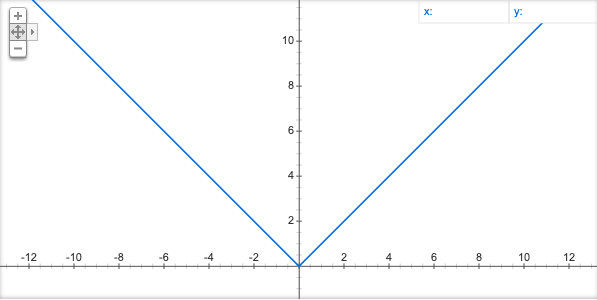
\includegraphics[scale=0.25]{graph.png}}
\end{columns}
\end{frame}

\begin{frame}{Parent functions} \vspace{4pt}
you should be able to identify by name and sketch a graph of each of the following parent functions.
    \begin{enumerate}
    \begin{multicols}{3}
        
   
        \item $y=x$
         \item $y=|x|$
          \item $y=x^2$
           \item $y=x^3$
           \onslide<2->{
            \item $y=x^b$
             \item $y=\sqrt{x}$
              \item $y=\sqrt{3}{x}$
               \item $y=\frac{1}{x}$}
               \onslide<3->{
                \item $y=\sin x$
                 \item $y=\cos x$
                  \item $y=\tan x$
                  \item $y=\Ln x$}
                  
                   \end{multicols}
    \end{enumerate}
\end{frame}

\begin{frame}[standout]
    \flushleft
\begin{center} Thank you \\
\textbf{Github repository address}:\\
\textcolor{purple} {https://github.com/RonakRah/overleaf1}
\end{center}
\end{frame}

\end{document}